\documentclass[conference, twocolumn]{IEEEtran}

\usepackage[english,french]{babel}
\usepackage{graphicx}
\usepackage{color} 
\usepackage[colorlinks]{hyperref}
\usepackage{palatino, url, multicol}
\usepackage{psfrag}
\usepackage{subfigure}
\usepackage{amsthm}
\usepackage{amsfonts}
\usepackage{amsmath}
\usepackage{algorithmic}
\usepackage{algorithm}

%\pdfpagewidth 8.5in
%\pdfpageheight 14in 

\theoremstyle{definition}

\newtheorem{definition}{Definition}[section]
\newtheorem{example}{Example}[section]

\hyphenation{op-tical net-works semi-conduc-tor}


\begin{document}

\title{On-Time Network On-Chip}

%\author{Dai Bui, Alessandro Pinto \\
%	Center for Hybrid and Embedded Software Systems, EECS \\
%    University of California, Berkeley \\
%    Berkeley, CA 94720, USA \\
%    \{\tt daib, pinto\}@eecs.berkeley.edu
%}

\maketitle

%\IEEEpeerreviewmaketitle
\begin{abstract}
Multi-core and many-core have become the major trend in processor development.
However, the more cores, the more communication unpredictability. One
question is how to use multi-core and many-core in real-time embedded systems?
How does a critical application know for sure that one packet sent from a node
will reach the destination node within a certain amount of time? In such a
case, faster does not always imply better. In multi-core, communication is
often more expensive than computation. The communication overhead often
greatly reduces the performance of a parallel application. An explicit
communication mechanism between cores running critical tasks is also a must.
This mechanism needs to be simple yet efficient and flexible enough for most of
applications.

In this paper, we provide a detailed delay analysis of multiplexing of real-time
channels in worm-hole flow control for network on chip then use a cycle
accurate simulation platform to prove the worst-case delay estimation and
deadline-based packet scheduling algorithm.

\end{abstract}

\section{Introduction}
Network on chip has become an important paradigm today
~\cite{DallyPacketNotWire}. As a network on chip gets larger, the communication on the network becomes very complicated. Congestions on that network can occur
resulting in unpredictable delay in communications between network nodes. This non-deterministic behavior 
makes it very difficult to verify the timing semantics of a network on chip 
system, as a result, network on chip systems become unsuitable for real-time 
applications, especially critical control applications.

\begin{figure}[htp]
\centering
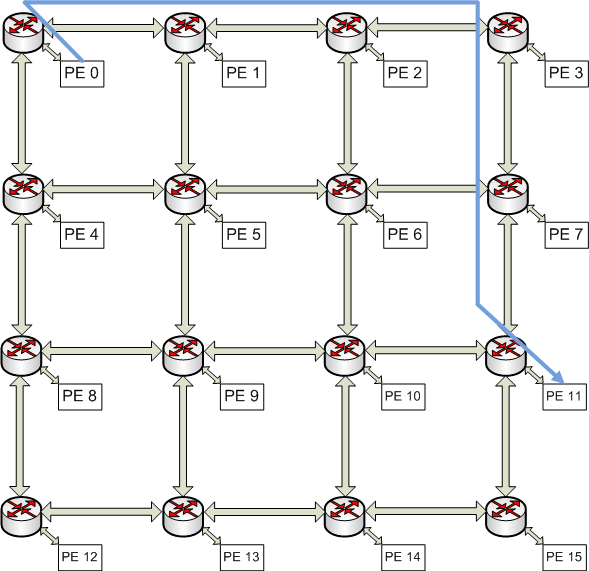
\includegraphics[width=7cm]{pics/NoC0}
\caption[Demand for a hard real-time flow.]
{How can a sending node make sure about the bounded delay for
a packet?}\label{fig:NoCRt}
\end{figure}

Our purpose is to bring the real-time communication to network on chip so that 
users can always guarantee deterministic behaviors of a critical system. To do 
so, it requires bounded delay communications between nodes in the network. 
For example, in Figure \ref{fig:NoCRt}, when processing element $0$ wants
to send a critical control packet p to processing element $11$, how can it know
for sure that the packet will reach the destination within a certain amount of time? 

%FIXME
%Structure of the paper

\section{Background}
\subsection{Network on Chip}
In a system on-chip, instead of connecting modules directly by dedicated wire,
they are connected by a packet switch network. Our experimental network, as
in Figure \ref{fig:NoCRt}, is a 2D mesh network. At each node of the mesh, a
processing element is connected to a router.

%packet figure
\subsection{Allocation Units}
A packet is further divided into {\em flits} to transmit
~\cite{DallyPrinNetwork}. The position of a flit determines if the flit is {\em
head, body} or {\em tail} flit. Only head flits contain routing information for
packets, body and tail flits follow head flits on the same path from sources to
destinations.
\subsection{Flow Control Schemes}
Networks are classified into several types based on how their resources are
allocated to packets on the networks. Following are three popular flow control
schemes:
\subsubsection{Store-and-Forward}
In store-and-forward flow control scheme, a packet has to be received entirely
before being forwarded. This flow control scheme gives longer end-to-end delay
in comparison with the following flow control schemes.
\subsubsection{Virtual-Cut-Through}
In virtual-cut-through scheme, a packet does not need to be received entirely
before being forwarded, however, receiving nodes is required to have enough
buffer space for incoming packets.
\subsubsection{Worm-Hole}
In worm-hole flow control, receiving nodes do not need to have enough buffer
space for incoming packets. Instead, packets are divided into flits and flits
are pipelined through networks. We will employ this flow control scheme in our
design.
\section{Related Work}
\subsection{\AE thereal}
This work ~\cite{Goossens_chapter4} is from NXP. This architecture tries to
avoid contention using contention-free routing by {\em delaying} some packets. \AE
thereal design tries to minimize the area of routers by minimizing buffer
spaces. This design purpose makes \AE thereal very suitable for small and less
complicated systems.

Guaranteed packets are multiplexed using TDMA by {\em global} scheduling of
packet injection ~\cite{Moonen07SPRINGER} from network interfaces to
routers. This mechanism makes systems based on this architecture less
{\em flexible} and {\em scalable} since as the number of components in a network
on chip grows larger, it is very difficult to find a suitable and efficient {global  scheduling} algorithm.
Furthermore, the TDMA slot allocation is currently solved at {\em design time}
to optimize the system ~\cite{Moonen07SPRINGER}, resulting in a number of
configurations and these configurations are programmed (or loaded) in the
network on chip. \AE thereal routers are often configured at design-time so
minimize the size of routers by removing slot tables, which could be very large
for a large network. This router optimization makes this architecture unable to
exploit multiple paths from source to destination to avoid conflicts between
guaranteed service packets. \AE thereal also has some known issues with bursty
traffic ~\cite{Hansson07ISSS}, which is typical in multi-core.

The above problems make \AE thereal unsuitable for systems requiring
flexibility and scalability like multi-core.

\subsection{SoCBUS}
SoCBUS architecture ~\cite{SoCBUS} is from Linkoping University. It seeks to 
guarantee real-time properties by setting up a path before ending:
\begin{itemize}
\item Initiate a path by sending a setting up packet.
\item The path will be {\em blocked} until all data have been sent.
\item After that the path is unlocked
\end{itemize}
This approach has the following problems: 
\begin{itemize}
\item What happens if we have two real-time paths on the same link?
\item Other traffic sharing a link with this real-time path is blocked while 
data is sent. This seems to be a good solution when sending a large bulk of data 
but not good for periodic, non-continuous flows.
\item Utilization of this approach can be low if real-time flows only require
low bandwidth.
\end{itemize}
\subsection{QNoC}
This work is from Technion ~\cite{QNoC}. Packets are sent synchronously. 
This architecture supports multi service levels as in Table
\ref{table:QNoCTable}.

\begin{table}[htbp]
\begin{center}
  \begin{tabular}{ | p{2.3cm} | p{4cm} | p{1.2cm} |}
    \hline
	Service-Level & Description & Priority \\ \hline
	Signaling & Urgent Messages, Short Packets, Interrupts, Control signals 
	requiring low transport latency & Highest \\ \hline
	Real-Time & Real-time and streaming packets & \\ \hline
	RD/WR & Short memory and register access & \\ \hline
	Block Transfer & Long messages and blocks of data & Lowest \\
    \hline
  \end{tabular}
\end{center}
\caption{QNoC Service Levels}
\label{table:QNoCTable}
\end{table}

This seems to be a good approach for soft real-time applications like video streaming
but this is not really suited for hard real-time applications since what happens 
when multiple real-time flows have to share the same link:
\begin{itemize}
\item Non-deterministic behaviors for flows.
\item Signaling packets can block real-time packets.
\end{itemize}
To solve this problem, we need to keep track of the number and specifications of
real-time flows on a link to make sure that the link is never overloaded.

\section{Flexible and Verifiable On-time Network on Chip}
The real-time communication between some nodes in a network 
on a chip can be achieved by borrowing the resource reservation idea
~\cite{Zhang93rsvp} from the Internet to the network on chip. In that, all the
real-time communications have to be previously reserved on the network. 

Real-time flows can be multiplexed ~\cite{Ferrari90ascheme}~\cite{ZhangService}
on links in networks without violating real-time requirements. Other best-effort
flows can still use remaining bandwidth on reserved links.

An admission control mechanism is implemented, thus when a reservation 
for a real-time flow is initiated by a sender in a network, the network will determine if 
it can accept that reservation or not based on its current state of other 
reservations of other real-time flows on the network.

\begin{figure}[htbp]
\centering
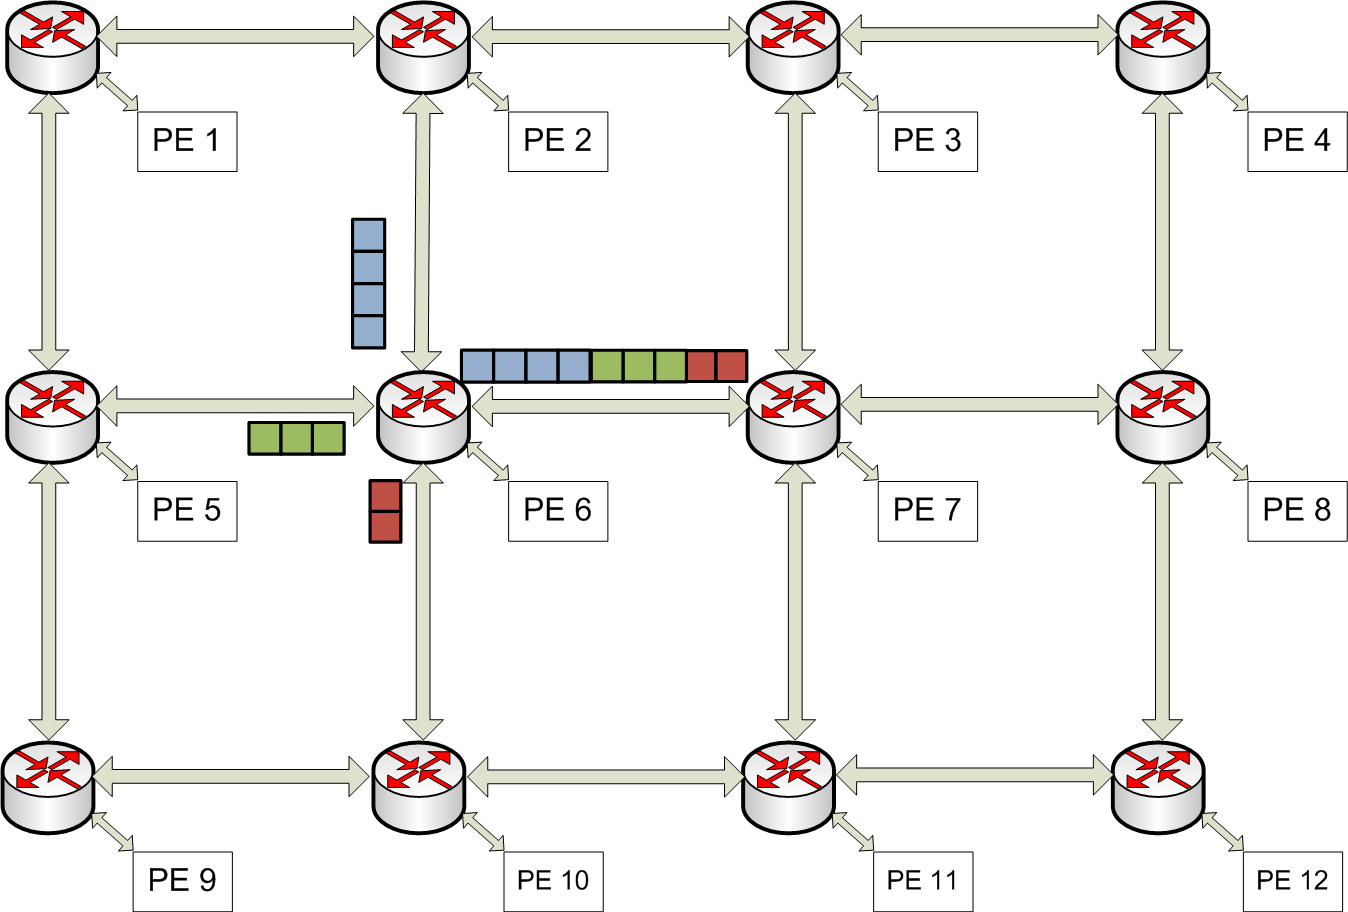
\includegraphics[width=7cm]{pics/Multiplex2}
\caption[Real time flow multiplexing.]
{Real-time flow multiplexing.}\label{fig:FlowMultiplex}
\end{figure}

We set design goals for our network on chip:
\begin{itemize}
\item Multiple real-time flows can be multiplexed on one link
~\cite{Ferrari90ascheme} as in Figure \ref{fig:FlowMultiplex}.
\item Utilize the spatial data paths between sources and nodes to avoid the 
conflicts between real-time flows.
\item Does not block links completely as SoCBUS \cite{SoCBUS}, best-effort flows 
still can travel links used by real-time flows.
\item Avoid unpredicted behaviors networks as in QNoC ~\cite{QNoC}, when there
are multiple real-time flows suddenly travelling on the same link and their total bandwidth 
exceeds the bandwidth of the link. The admission control in our architecture can 
prevent that. Senders should always know if their required specifications for 
their communications can be met or not. 
\item Provide maximum flexibility and scalability to applications, no specific
configuration is done at {\em design time} as in \AE thereal ~\cite{Moonen07SPRINGER}. The
new architecture also needs to avoid {\em global scheduling} problem since this
makes a network on chip difficult to be dynamically reconfigured effectively.
\end{itemize}

\section{Definitions}
$\mathbf{N}$ is the set of interger values.

$T \subseteq \mathbf{N}$ is the set of the minimum interval values between
packets of flows.

$L \subseteq \mathbf{N}$ is the set of packet lengths.

$D \subseteq \mathbf{N}$ is the set of packet delays of real-time flows.

$\mathcal{V} \subseteq \mathbf{N}$ is the set of virtual channels between pairs of nodes.

$C$ is the set of {\em cores} on the on-chip network.

$R$ is the set of {\em routers}.

Then the set of {\em nodes} on the network is defined as:
\begin{equation}\label{reio}
V = C \cup R
\end{equation}
And $E$ defined as:
\begin{equation}
E \subseteq V \times V 
\end{equation}
is the set of {\em directed edges} between nodes in the network.

The set of {\em  real-time flows} on the network is defined as:
\begin{equation}
F \subseteq C \times C \times \mathcal{V} 
\end{equation}

And $P$ is a {\em mapping } between a real-time flow with its specifications:
\begin{equation}
P:F \rightarrow \tau \times T \times L \times D
\end{equation}
in which $\tau$ is the set of packet types.

$t_f$ is the {\em minimum} packet interval time in {\em cycles} between
two successive packets of a real-time flow $f$.

$l_f$ is the {\em maximum} length of a packet in {\em flits} of real-time
flow $f$.

$s_{f,e}$ is the service time for a packet in a node including header 
processing, transmission time, and any other operations. $s$ is often a 
function of $l$: $s_{g,e}=f(l_g)$. We can set $s_{f,e}=value(l_f)$, this means
that it takes $1$ cycle for a router to process and send one flit over a link. In pipeline router
model as in ~\cite{PehDelayModel}~\cite{PehSpecPipeR}, some
pipeline stages is added to $l$ to form $s$.

$d_f$ is the {\em worst case} end-to-end delay of a packet of real-time flow
$f$.

$q_{f,v}$ is the {\em maximum} delay in cycles of a {\em flit} in
flow $f$ at node $v$.This is the {\em queueing} delay. The local delay ({\em
queueing} delay) at each node of a packet is defined as the duration from the
{\em header} of that  packet is received until the header is started to send.
We do not need to include the service time of the packet itself at the node.
The {\em maximum} local delay of a packet of a flow $f$ at a node is thus the
same as the maximum delay of a flit of flow $f$ at the same node since we do
not allow real-time packet pre-emption. % In \cite{Ferrari90ascheme}, the delay is :

%\begin{equation}\label{equ:nodedelay1}
%q_{i,n} = \sum_{j=1}^{i-1}s_{j,n}+s_{max} \forall i = 1, ..., K
%\end{equation}

$p_{f,e}$ is the {\em propagation} delay in cycles of a {\em flit} or
a {\em packet}, since real-time packets are not preemptible, of real-time flow
$f$ on link $e \in E$. We assume in our network on chip, $p_{f,e}=1 \forall e \in E$.

% $r_{v,f,h}$ is the time of flit $h$ of flow $f$ reaches node $v$.  

$d_{f,e}$ is the {\em maximum} delay of a flit of flow $f$ on link $e \in E,
e=(v,u)$ measured in cycles. This delay is the duration between the time a flit
reaches the source node $v$ and the time the flit reach the destination node
$u$ of that link $e$.

\begin{equation}\label{equ:edgeDelay}
d_{f,e} = q_{f,v} + p_{f,e} = q_{f,v} + 1 
\end{equation}

% and
% 
% \begin{equation} 
% d_{f,e_{v,u}} \geq r_{u,f,h} - r_{v,f,h}
% \end{equation}

\begin{equation}
y_{f,e} = \left\{ \begin{array}{lrc}
1 \mbox{ if flow } f \in F \mbox{ uses link } e \in E \\
0 \mbox{ otherwise} 
\end{array}\right.
\end{equation}


% \begin{equation}
% \delta_{f,v} = \left\{ \begin{array}{lrc}
% 1 \mbox{ if flow } f \in F \mbox{ going through node } v \in V \\
% 0 \mbox{ otherwise} 
% \end{array}\right.
% \end{equation}

% \begin{eqnarray}
% \sigma_{f,e} = \left\{ \begin{array}{lrc}
% 1 \mbox{ if flow } f \in F \mbox{ has the largest maximum} \\
% \mbox{packet length of all flows on } e \in V \\ 
% 0 \mbox{ otherwise} 
% \end{array}\right.
% \end{eqnarray}

\begin{equation}
I_{v,e} = \left\{ \begin{array}{lrc}
1 \mbox{ if } e \in E \mbox{ is outgoing edge from } v \in V \\
-1 \mbox{ if } e \in E \mbox{ is incoming edge from } v \in V \\
0 \mbox{ otherwise}
\end{array}\right. 
\end{equation}

$\forall f=(s, d, id) \in F$  let $b$ be a vector s.t. $b_f(s) = 1$, 
$b_f(d) = -1$ and $b_f(i) = 0, \forall i \in C \mbox{ and } i \neq s, d$,
 then we have $Iy_f=b_f$, this condition is for unique path between $s$ and $d$.

A valid configuration ${\mathcal{C}}(F)=(P, \lbrace y_{f,e}:f \in F, e \in E
\rbrace )$.

\section{Architecture}
\subsection{Programming Model}
\subsubsection{Network Stack Model}
At each node in a router, we employ the Internet stack to each node in the 
network on chip as in Table \ref{table:NetworkStack}.
\begin{table}[h]
\begin{center}
  \begin{tabular}{ | l | }
    \hline
    Application layer at processing units \\ \hline
    Transport layer at processing units \\ \hline
    Network layer at routers \\ \hline
	Data link layer at routers \\ \hline
	Physical layer \\
    \hline
  \end{tabular}
\end{center}
\caption{Network stack model}
\label{table:NetworkStack}
\end{table}

\subsubsection{Configuration: Distributed vs. Centralized}
Since our purpose is to design a distributed network on chip system, thus the
configurations of the network can be dynamically changed at {\em run-time}.
This requirement makes the distributed configuration scheme unsuitable since,
for instant, when there are two requests for real-time flows, we maybe have to
reduce the {\em slack} of other flows, however it is difficult to reduce the
slack of a flow {\em concurrently} in a distributed manner by two or more
requests for real-time flows without making the end-to-end delay of the
modified flow inviolate its requirement. We choose to use centralized scheme
since we can reduce the overhead of distributed routing and we can more easily
implement more complicated routing algorithm to balance and optimize a network
on chip.

\subsection{Path Setup Protocol}
When in need of a real-time communication, the processing unit at each node 
will issue a request for setting up a path:

{\em Setuppath.request(source\_id, destination\_id, virtual\_channel\_id T, L,
D);}

\begin{figure}[htp]
\centering
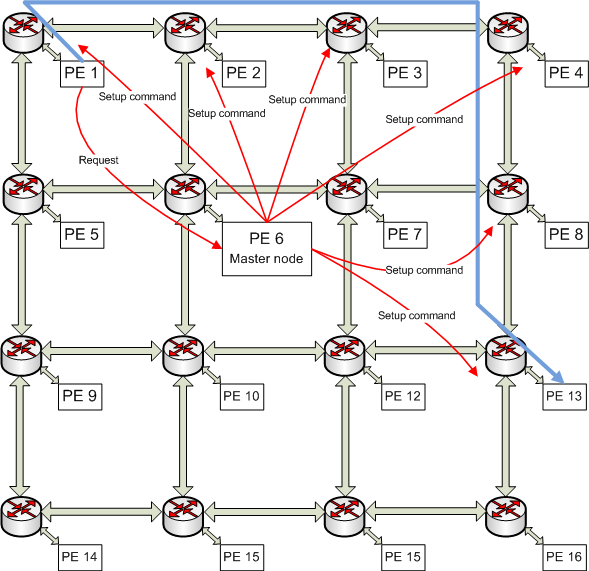
\includegraphics[width=7cm]{pics/Protocol2}
\caption[Setup request for a real-time flow.]
{Real-time flow setup protocol.}\label{fig:ReqSetup}
\end{figure}

This request will be sent over the network by a REQ message to a specific node
in the network, called {\em master node}, as in Figure \ref{fig:ReqSetup}.
Based on its knowledge about other flows in the network and the demand for the
new real-time flow, the master node will seek to find a suitable path. If there
exists a suitable path, the master node will send SETUP command messages to
appropriate routers in the network to configure routers' configurations. This
re-configuration can include adjusting configurations of other flows at the routers.

Routers receiving SETUP command message will adjust their internal
configurations as specified in the message. After finishing setting up internal
configurations, routers will send back an acknowledgement ACK message to
the master node. When the master node have received all its expected ACK
messages from routers, it sends an ACCEPT message to the requesting node
(node requested a new real-time flow). The requesting node can start sending
data after receiving that ACCEPT message.

If the master node cannot find a suitable path, it sends back to the requesting
node a REJECT message saying that new real-time flow cannot be set up on the
network.

So the setting up path response can be: ACCEPT, REJECT

When a path is not needed, it can be torn using path-tearup protocol, which
works basically as the path-setup protocol but with reversed commands.

\subsection{Design Questions}
\begin{itemize}
\item Should we specify the path directly in this request? Static initialization 
can be useful in some programming model like Giotto.	
\item Is it possible that the acceptance message will be blocked on the network 
or it reaches the source too late? We should give priority to such kind of control
message.
\item Real-time flows block other best-effort packets traveling on the link when 
the utilization of all the packets on the link is $1$. We need a mechanism to
reroute all best-effort packets.
\end{itemize}

To reduce the size of each router, we can use processing elements to do 
complicated tasks like calculating admission criteria for a new flow at each node 
and rerouting for finding a new suitable path on a network.


One characteristic of this scheme is that the buffer for each 
real-time flow at each node is bounded ~\cite{Ferrari90ascheme}, and thus
real-time packets can be sent {\em asynchronously} resulting in better bandwidth
since we do not have to send {\em acknowledgement} for each flit sent. So at
data link layer, we employ heterogeneity communications, {\em synchronous}
communications for best effort packets and {\em asynchronous} communications
for real-time packets as in Figure \ref{fig:HeteroComm}. Best-effort packets
are preemptible by real-time packets. Real-time packets are not preemptible.
Since real-time flits does not need acknowledgement so the speed of sending
real-time packets is two time faster than best-effort packets.


\begin{figure}[htbp]
\centering
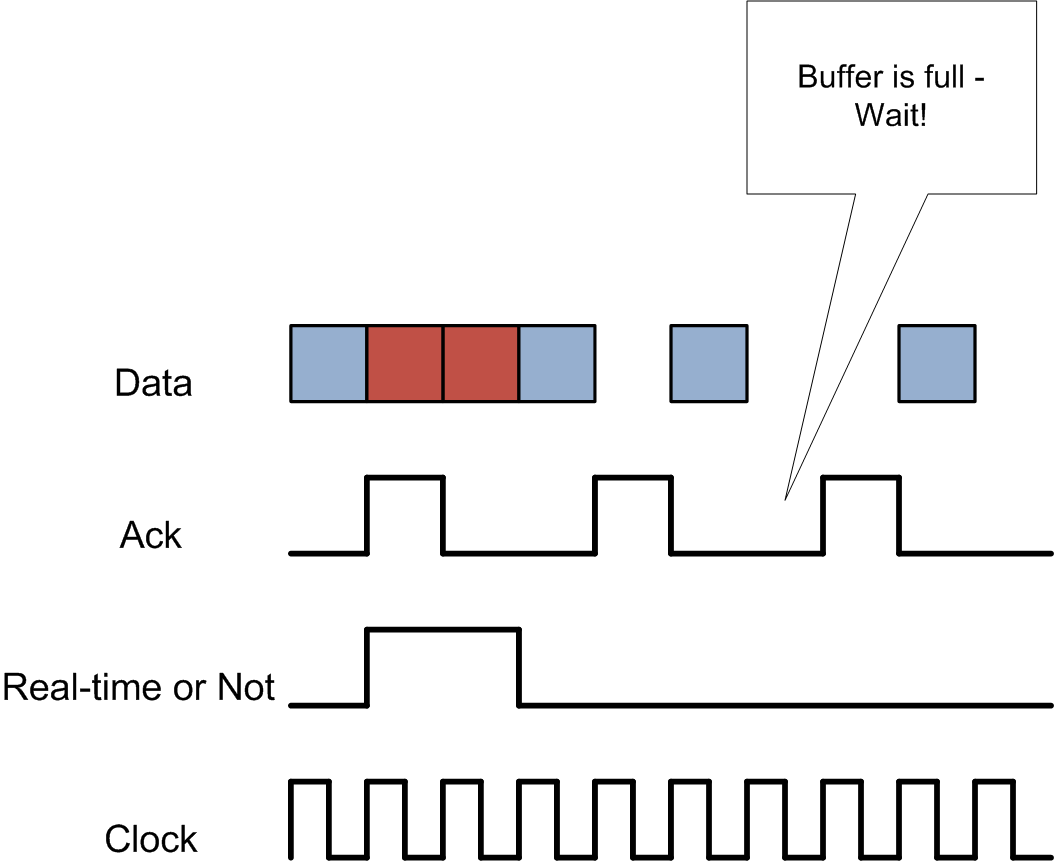
\includegraphics[width=8cm]{pics/HeteroComm.png}
\caption[Heterogeneous Communication for Packets.]
{Real-time packets and best-effort packets are treated
differently.}\label{fig:HeteroComm}
\end{figure}

\section{System Analysis}
\subsection{Packet Scheduling}
At each node, we use Earliest Due Date (EDD)
~\cite{VermaJitter91}~\cite{LiuSchedulingRT} to schedule packets, the deadline
for each packet of flow $f$ at node $n^{th}$ is computed as follows:
\begin{equation}\label{equ:deadline1}
dl_{f,n}=t_0 + \sum_{k=1}^{n}q_{f,k}+P_n
\end{equation}
where $t_0$ is the time the packet is sent from the source and $P_n$ is the propagation
delay from the source till node $n^{th}$ (communication time). We set
$P_n=n$ since we assume that our in network on chip, it takes one cycle for a
head flit to travel between two successive nodes. Thus, (\ref{equ:deadline1}) becomes:

\begin{equation}\label{equ:deadline2}
dl_{f,n}=t_0 + \sum_{k=1}^{n}d_{i,k}
\end{equation}

\subsection{Delay Model Analysis}

The delay model in ~\cite{Ferrari90ascheme}~\cite{VermaJitter91} is
for store-and-forward flow control. However we will use worm-hole flow
control since it has better throughput.

%{\textbf{Definitions:}}

Similarly to ~\cite{Ferrari90ascheme}, if we assume that all $K$ 
real-time flows going through link $e$ satisfy the following condition:
\begin{equation}\label{equ:intervalservice1}
t_f \geq \sum_{j=1}^Ks_{j,e}, \forall f = 1,...,K
\end{equation}

We assume that one flit will be transmitted over a link $e \in E$ in one cycle
then $s_{f,e}=value(l_f), \forall f \in F$. So (\ref{equ:intervalservice1})
becomes:

\begin{equation}\label{equ:intervalservice2}
t_f \geq \sum_{j=1}^Kvalue(l_j), \forall f = 1,...,K
\end{equation}

This means that {\em no deadlines} for subsequent packets of a real-time flow
will fall within the interval between time $t_0$ and $t_0 + \sum s = t_0 +
\sum_{j=1}^Kvalue(l_j)$.

We define a function $order_{e_{v,u}}(f)$ over the set of all real-time flows
$F$ as a function to determine if there are two packets $p_1$ and $p_2$, arriving at
a node $v$ at the same time of two real-time flows $f_1$ and $f_2$ respectively
and competing for an output link $e$, packet $p_1$ will be sent before $p_2$ if
$order_{e_{v,u}}(f_1) < order_{e_{v,u}}(f_2)$. 

\begin{figure}[htbp]
\centering
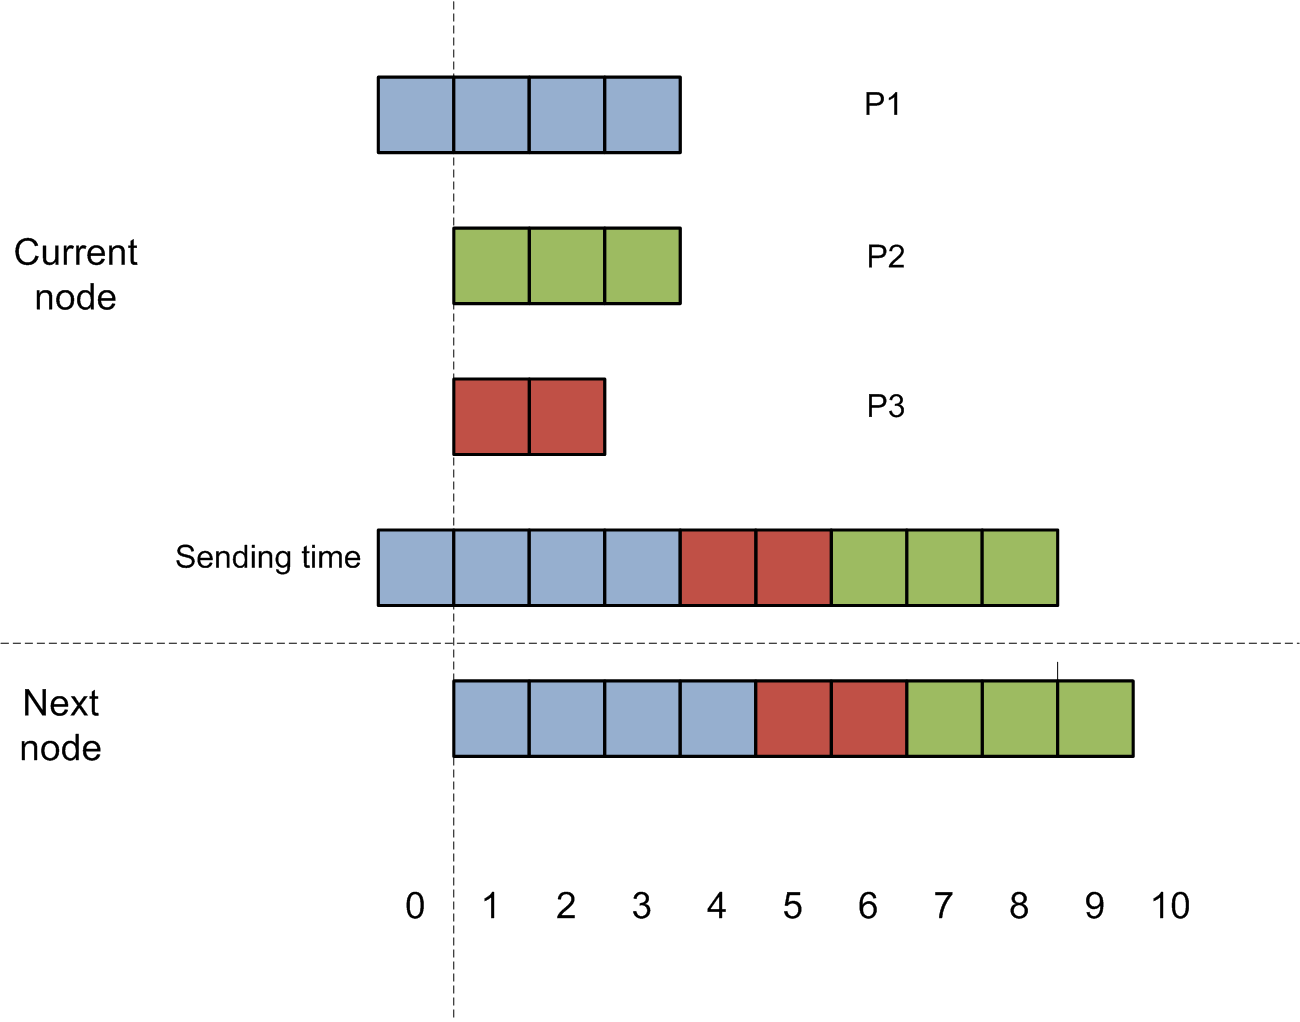
\includegraphics[width=8cm]{pics/DelayModel.png}
\caption[Delays for packets.]
{Delay Model.}\label{fig:DelayModel}
\end{figure}

In worm-hole flow control scheme, the local delay at each node is a little bit
different from ~\cite{Ferrari90ascheme}. For an edge $e = (v,u)$, we have:

\begin{eqnarray}\label{equ:queueDelay}
q_{f,v}y_{f,e} \geq \sum_{g \in F:order_{e}(g) <
order_{e}(f)}s_{g,e}y_{g,e} + \notag \\ 
max_{order_{e}(i)>order_{e}(f)}(s_{i,e}y_{i,e})-1, \forall e = (v,u)
\in E
\end{eqnarray}

In the (\ref{equ:queueDelay}), the $y_{f,e}, y_{i,e}, y_{g,e}$ parameters mean
that flow $f, i, g$ share the same link $e$. The reason for
(\ref{equ:queueDelay}) is that the maximum local (queueing) delay  that a packet
$p$ of flow $f$ on a link $e$ is the total time to send all packets of other
flows of higher priorities plus  the time  to send the {\em biggest
possible rest} of one packet of flows with {\em lower} priorities since real-t
ime packets are not pre-emptible.

For example, from Figure \ref{fig:DelayModel}, if we suppose $p_i$ is a packet
of flow $f_i$, and $order_{e}(f_1) < order_{e}(f_2) < order_{e}(f_3)$, then we can easily see that
the bounded {\em queueing} delay for packets $p_1$ and $p_2$ are 3 and 5
respectively as computed by equation (\ref{equ:queueDelay}). However, the
bounded queueing delay for packet $p_3$ is 5 if it comes at the same time as $p_1$ and $p_2$.

From (\ref{equ:edgeDelay})(\ref{equ:queueDelay}) and delay on
each edge is set as small as possible:

\begin{eqnarray}\label{equ:edgeDelay2}
d_{f,e}y_{f,e} = \sum_{g \in F:order_e(g) < order_e(f)}s_{f,e}y_{f,e} +
\notag\\  
max_{order_{e}(i)>order_{e}(f)}(s_{i,e}y_{i,e}), \forall e \in E
\end{eqnarray}

For different applications, choose different {\em order} functions can be
chosen. In this paper, to minimize the total local delay at each node, we
choose a scheduling scheme that forwards packets of flows that have smallest maximum
packet length first by setting $order_{v,e}(f)=l_f$, then
(\ref{equ:edgeDelay2}) becomes:

\begin{eqnarray}\label{equ:edgeDelayPacketLength}
d_{f,e}y_{f,e} = \sum_{g \in F:l_g <
l_f}s_{g,e}y_{g,e} +max_{l_i>l_f}(s_{i,e}y_{i,e}), \forall e \in E
\end{eqnarray}

This means that flows with smaller maximum packet lengths will be given smaller
delays at this node (thereby smaller deadlines when packets come at the same
time).

However, from (\ref{equ:edgeDelayPacketLength}), it is possible to see that
there is some case, at a node, the bounded delay of flow $f$ with the largest packet length
will be {\em smaller} than the bounded delay of some other flow with smaller
maximum packet length. To still use (\ref{equ:deadline2}) for scheduling, we
have to assign a {\em virtual delay} for the flow $f$ so that the {\em virtual deadline},
computed from (\ref{equ:deadline2}), is greater than that of any other flows to
make sure that, if all the packets of all flows come at the same time, the
packet of the flow $f$. We will prove that, this virtual delay scheme for the
flow {\em does not} make any packet of the flow miss its deadline and the delay
bound of a packet is still the same as in (\ref{equ:edgeDelayPacketLength}).
This virtual delay is set to the largest bounded delay of all other flows
sharing the same link.

{\textbf{Theorem 1:}} {\em  The above virtual delay scheme never makes
packets of flow $f$ miss their real deadlines computed from
(\ref{equ:deadline2}) and (\ref{equ:edgeDelayPacketLength})}.

{\em Proof:} Suppose that $\mathcal{S}$ is the total maximum service time of all
other flows except $f$. So the real delay bound of $f$ is ${\mathcal S}+1$.
Suppose that a packet $p$ of $f$ comes at time $t_0$, then the {\em real}
deadline for the packet is $t_0+{\mathcal S}+1$. Since from
(\ref{equ:intervalservice2}), each flow can not have more than 1
packet deadline in the duration $(t_0, t_0+{\mathcal S}+1)$. If in
$(t_0, t_0+{\mathcal S}-1)$, there is any cycle that no flit of other packets is
sent, then the scheduler will immediately start forwarding packet $p$ of flow $f$.
Otherwise, at time $t_0+{\mathcal S}$, all the flits of other packets are
forwarded, then the packet $p$ is started forwarding and its header will reach
the next node at $t_0+{\mathcal S}+1$. The real delay bound is the same as
estimated by (\ref{equ:edgeDelayPacketLength}).

\subsection{Configuration}
A valid configuration ${\mathcal C}(F)$ must satisfy
(\ref{equ:intervalservice2})(\ref{connectivity1}) (\ref{equ:e2eDelayST})(\ref{equ:utilization1})

\begin{equation}\label{connectivity1} Iy_f=b_f,\forall f \in F
\end{equation}

From ~\cite{Ferrari90ascheme},the total delay at each hop of a real-time flow
has to satisfy the delay constraint of the real-time flow.

\begin{equation}\label{equ:e2eDelayST}
\sum_{e \in E}d_{f,e}y_{f,e} \leq d_f, \forall f \in F
\end{equation}

When multiple real-time flows share the same link, the following conditions
 have to be met on each shared link ~\cite{Ferrari90ascheme}~\cite{VermaJitter91}:

\begin{equation}\label{equ:utilization1}
\sum_{f \in F}\frac{s_{f,e}}{t_f}y_{f,e} \leq 1, \forall e \in E
\end{equation}

Since $s$ is a function of the packet length, for a simple (non-pipeline) router
model, we often have $s_{g,e}=value(l_g) \forall f \in F$, then
(\ref{equ:utilization1}) becomes:

\begin{equation}\label{equ:utilization2}
\sum_{f \in F}\frac{value(l_f)}{t_f}y_{f,e} \leq 1, \forall e \in E
\end{equation}

However (\ref{equ:e2eDelayST}) is for a store-and-forward flow control, in
worm-hole flow control, it becomes:
\begin{equation}\label{equ:e2eDelayCT}
\sum_{e \in E}d_{f,e}y_{f,e} + (s_{f,last\_edge} - 1) \leq d_f, \forall f \in F
\end{equation}
since we have to include the service time, $s_{f,last\_edge}-1$, for each
packet so that the last node can receive the {\em remaining} flits in a
packet of flow $f$, not only the header of the packet.

%\begin{equation}\label{equ:e2eDelayCTNonPipeline}
%\sum_{e \in E}d_{f,e}y_{f,e} + l_f - 1 \leq d_f, \forall f \in F
%\end{equation}

From (\ref{equ:edgeDelayPacketLength})(\ref{equ:e2eDelayCT}) we have:
\begin{eqnarray}\label{equ:e2eDelayCTNonPipeline1}
\sum_{e \in E} \Biggl(\sum_{g \in F:l_g <
l_f}y_{g,e}s_{g,e} +max_{l_i>l_f}(s_{i,e}y_{i,e})\Biggr)\notag \\ \leq
d_f-s_{f,last\_edge} + 1, \forall f \in F
\end{eqnarray}

For simple router models (non-pipeline), we have $s_{f,e} = value(l_f),\forall e
\in E$, then (\ref{equ:e2eDelayCTNonPipeline1}) becomes:

\begin{eqnarray}\label{equ:e2eDelayCTNonPipeline2}
\sum_{e \in E} \Biggl(\sum_{g \in F:l_g <
l_f}y_{g,e}value(l_g) +max_{l_i>l_f}(value(l_i)y_{i,e})\Biggr)\notag \\ \leq
d_f-value(l_f) + 1, \forall f \in F
\end{eqnarray}

Now a valid configuration ${\mathcal C}(F)$ has to satisfy
(\ref{equ:intervalservice2})(\ref{connectivity1}) (\ref{equ:utilization2})
(\ref{equ:e2eDelayCTNonPipeline2})

\subsection{Dynamic Path Establishment and Routing}
When a new real-time path needs to be set up with some specifications, we have:
$F \rightarrow F \cup \{f^{'} \}=F^{'}$
and $T \rightarrow T^{'}$ s.t. $T^{'} (f)=T(f)\forall f \in F$ and $T^{'}
(f^{'})=(\tau ^{'}, T^{'}, L^{'}, D^{'})$.

The problem becomes: Find $y_{f^{'}e}$ s.t. ${\mathcal C}(F^{'})$ is valid
when we know that ${\mathcal C}(F)$ is valid.

For a new configuration ${\mathcal C}(F^{'})$, we find a new flow $f^{'}$ such
that the conditions (\ref{connectivity1})(\ref{equ:utilization2}) are satisfied. And
the path delay constraint from (\ref{equ:e2eDelayCTNonPipeline1}) is:

\begin{eqnarray}\label{equ:e2eDelayNewPath1}
\sum_{e \in E} \Biggl(\sum_{g \in F:l_g <
l_{f'}}value(l_g)y_{g,e} +max_{l_i>l_{f'}}(value(l_i)y_{i,e})\Biggr)\notag \\
\leq d_{f'}-value(l_f') + 1, \forall f' \in F
\end{eqnarray}

To add a new real-time flow like this to the network without modifying the paths
of other previous real-time flows, we store a {\em slack} of delay for each
real-time flow. Then whenever we add a new real-time flow and modify the local
bounded delay of other flows we check if the increasing delay amounts of the
flows exceed the slack of the flows and then recompute new slacks for these
flows. The slack of a flow $f$ is computed as:

\begin{eqnarray}\label{equ:slack1}
	slack_f= d_f-value(l_f) + 1 - \notag \\
	\sum_{e \in E} \Biggl(\sum_{g \in F:l_g < l_f}y_{g,e}value(l_g)
	+max_{l_i>l_f}(value(l_i)y_{i,e})\Biggr) \notag \\ 
	\forall f \in F
\end{eqnarray}

With this scheme, we have modifying the configurations of other flows sharing
the same link with the new flow. The master node will issue a SETUP command to
override the previous configurations at routers.

If a new flow $f'$ is requested, then employing {\em shortest maximum packet
length first} ordering requires to modify the delay of flows at sharing some
links with $f'$ that have larger maximum packet lengths larger than the new flow
maximum packet length. 

$\forall f \in F$  that $l_{f'} < l_f$ and $y_{f',e}y_{f,e}=1 \mbox{ for some }
e \in E$, from (\ref{equ:e2eDelayCTNonPipeline1}) we have:

\begin{eqnarray}\label{equ:e2eDelayModification}
\sum_{e \in E} \Biggl(\sum_{g \in F:l_g <
l_f}y_{g,e}s_{g,e}+y_{f',e}s_{f',e}+max_{l_i>l_f}(s_{i,e}y_{i,e})\Biggr)\notag
\\ \leq d_f-s_{f, last\_edge} + 1, \forall f \in F
\end{eqnarray}

or

\begin{eqnarray}\label{equ:e2eDelayModificatio2}
\sum_{\forall e \in E}y_{f',e}s_{f',e} \leq d_f-s_{f,last\_edge} + 1 - \notag \\ 
\sum_{e \in E} \Biggl(\sum_{g \in F:l_g <
l_f}y_{g,e}s_{g,e}+y_{f',e}s_{f',e}+max_{l_i>l_f}(s_{i,e}y_{i,e})\Biggr) \notag
\\ \forall f \in F
\end{eqnarray}

or

\begin{equation}\label{equ:e2eDelayModificatio3}
\sum_{\forall e \in E}y_{f',e}s_{f',e} \leq slack_f, \forall f \in F
\end{equation}

or

\begin{equation}\label{equ:e2eDelayModificatio4}
\sum_{\forall e \in E}y_{f',e}value(l_{f'}) \leq slack_f, \forall f \in F
\end{equation}

(\ref{equ:e2eDelayModificatio4}) is used as the criteria for any routing
algorithm to check if a new real-time flow can make any other existing
real-time flows on its path violate their end-to-end delay.

\section{Specifications}
\subsection{Message Structures}

There are two types of packets in best-effort flow identified by the head flit
in a packet. The head flit can be of CTRL (control) or HEAD (normal) type. The
structure of a REQ message (this is often a flit) to set up a real-time flow on the network is:

\begin{table}[htbp]
\begin{center}\resizebox{8cm}{!}{
  \begin{tabular}{ | l | l | l | l | l | l | l | l | }
    \hline
	CTRL & Req Node ID & Master Node ID & \multicolumn{2}{|c|}{REQ} \\ \hline
	BODY & Source ID & Destination ID & \multicolumn{2}{|c|}{$t_{min}$} \\ \hline 
	TAIL & \multicolumn{2}{|c|}{Flow ID} & $l_{max}$ & $d_{max}$ \\
    \hline
  \end{tabular}
}
\end{center}
\caption{REQ path message}
\label{table:PathMsg}
\end{table}

The SETUP message from the master node to router has the following structure:

\begin{table}[htbp]
\begin{center}\resizebox{8cm}{!}{
  \begin{tabular}{ | l | l | l | l | l | l | l | l | } 
    \hline 
	CTRL & Master ID & Router ID & SETUP & Virtual delay \\ \hline
	TAIL & \multicolumn{2}{|c|}{Flow ID} & Input gate & Output gate 	\\
    \hline
  \end{tabular}
}
\end{center}
\caption{SETUP path message}
\label{table:PathMsg}
\end{table}

The ACK or ACCEPT message has the following form:


\begin{table}[htbp]
\begin{center}\resizebox{8cm}{!}{
  \begin{tabular}{ | l | l | l | l | l | l | l | l | }
    \hline
	CTRL & Source ID & Destination ID & (ACK or ACCEPT) \\ \hline
	TAIL & \multicolumn{2}{|c|}{Flow ID} &  \\
    \hline
  \end{tabular}
}
\end{center}
\caption{SETUP path message}
\label{table:PathMsg}
\end{table}


The structure of a real-time data packet is:

\begin{table}[htbp]
\begin{center}{
  \begin{tabular}{ | l | l | l | l | l |}
    \hline
	HEAD & Flow ID & jitter & Data \\ \hline 
	BODY & \multicolumn{3}{|c|}{Data flit} \\ \hline
	BODY &\multicolumn{3}{|c|}{...} \\ \hline
	TAIL & \multicolumn{3}{|c|}{Data flit} \\
    \hline
  \end{tabular}
}
\end{center}
\caption{Real-time data message}
\label{table:DataMsg}
\end{table}

%\subsection{Considerations}

%\begin{figure}[htp]
% \centering
% 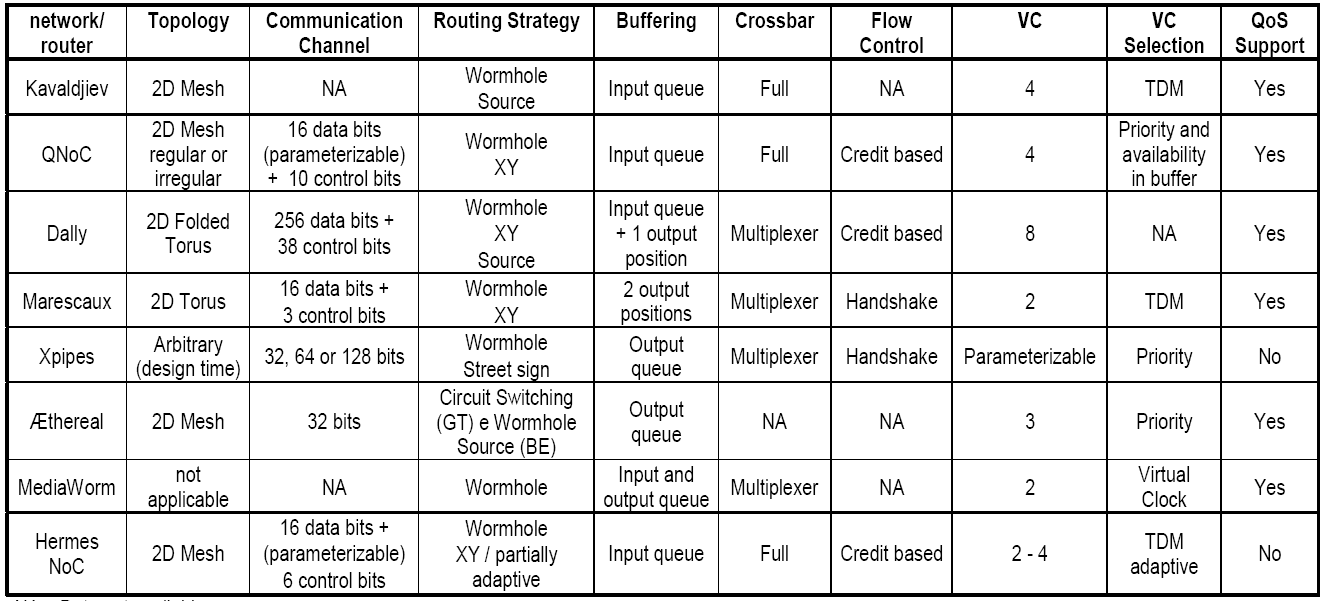
\includegraphics[width=8cm]{pics/OtherArcs.png}
% \caption[Other Spec.]
% {Specification of other network on chip architectures}\label{fig:otherSpec}
% \end{figure}
% 
% From this we can consider the format of a data packet since we have the 
% tradeoff between the length of a packet and the bounded delay of the packet. 
% If the packet is long, then our network is more efficient, however, the bounded 
% delay will probably large.

\subsection{Worm-hole Router Structure}
\subsubsection{Packet Identification}
In each real-time packet, the head flit contains a {\em unique flow
identification} number. A router will use this number to match the packet with
information of real-time flows it has in a table. If it can successfully find a
flow identification like that, the information about packets of that flows will
be loaded  for packet scheduling, including:
\begin{itemize}
  \item Input gate
  \item Output gate
  \item {\em Virtual} delay (for deadline-based packet scheduling)
  \item Real bounded delay (optional)
\end{itemize}

\subsubsection{Scheduling}
Figure \ref{fig:RouterStructure} shows the structure of a router. In a router,
each input has one {\em priority} queue for real-time packets of each output.
Packets in the priority queue are {\em ordered} by deadline as in
(\ref{equ:deadline2}). Each output will pick the top packets from priority
queues and compare their deadlines to find the packet with closest deadline and this
packet is selected to send. Best-effort packets are stored in FIFO queues as in
normal routers. The router is a cut-through router so that one packet can be
compared the deadline and forwarded right at the time its header each a node.

\begin{figure}[htp]
\centering
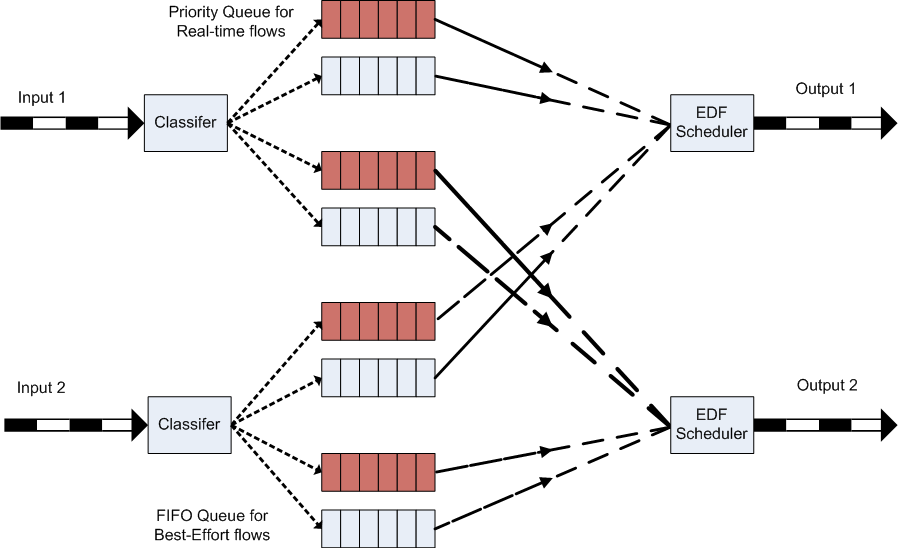
\includegraphics[width=8cm]{pics/Router.png}
\caption[Other Spec.]
{Structure of routers}\label{fig:RouterStructure}
\end{figure}

\subsection{Routing}

Several different routing algorithms can be implemented to optimize and balance
a network on chip like this depending on application requirements. In this
evaluation, we just implement an exhaustive depth-first search routing algorithm
to demonstrate the worst case delay estimation and our packet scheduling algorithm.

When a reservation algorithm of a path reaches a node and the calculated routing
link to another router cannot afford the service time and transmission rate or delay 
bound for that reserving flow. The master node monitors all configurations of
real-time flows on the network so various routing policy can be employed to
achieve better performance, delay, power and so on.

The routing algorithm is depth first search based on XY routing (try X
direction first). An example about routing is shown in Figure
\ref{fig:3FlowsEx} with three real-time flows. $Flow 1: PE7 \rightarrow
PE23, Flow 2: PE6 \rightarrow PE3, Flow 3: PE5 \rightarrow PE19$.

Flow 1 comes first and gets routed in blue path. Flow 2 comes later and gets
routed in read path.  When flow 2 gets routed through link from node 7 to node
8, the delay bound of flow 1 on that edge is modify, however, the total delay
bound of that flow still does not exceed the requested delay bound.

When flow 3 comes, it gets routed to node 7, however, it can not travel the
link from node 7 to 8 since the link utilization would exceed 1 if that link
has the third flow. The flow 3 then gets routed to node 12 then reachs the
destination node.

\begin{figure}[htp]
\centering
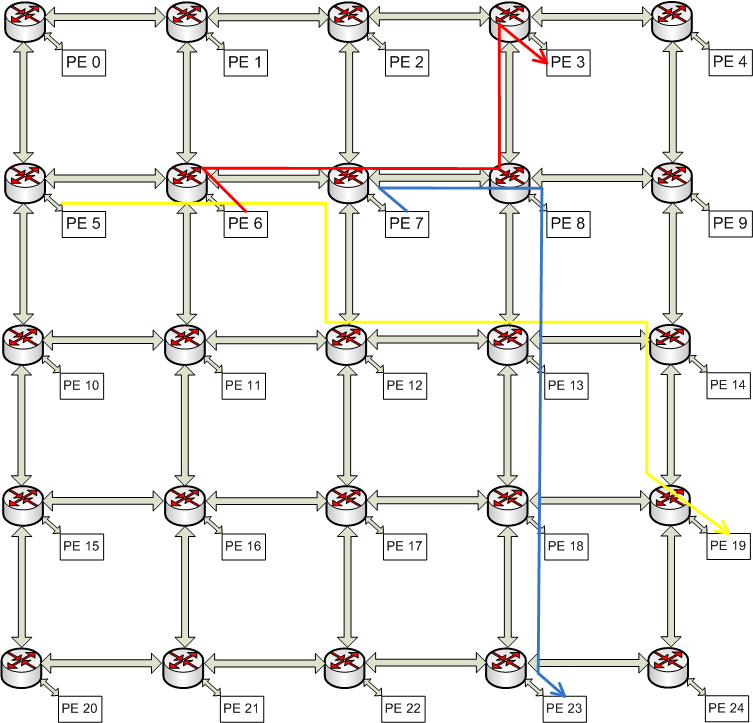
\includegraphics[width=8cm]{pics/Example.png}
\caption[Three flows example.]
{Example of three flows scheduled to share links}\label{fig:3FlowsEx}
\end{figure}

\section{Implementation}
Router micro-architecture can be implemented similarly as in
~\cite{Rexford98arouter}~\cite{ZhangService} and extend
~\cite{PehDelayModel}~\cite{PehSpecPipeR} to have better performance.

Simulation program is written in SystemC based loosely on Noxim ~\cite{Noxim}.
To test our implementation, we initiate three real-time flows on the network as
in Figure \ref{fig:3FlowsEx}.

\begin{figure}[htp]
\centering
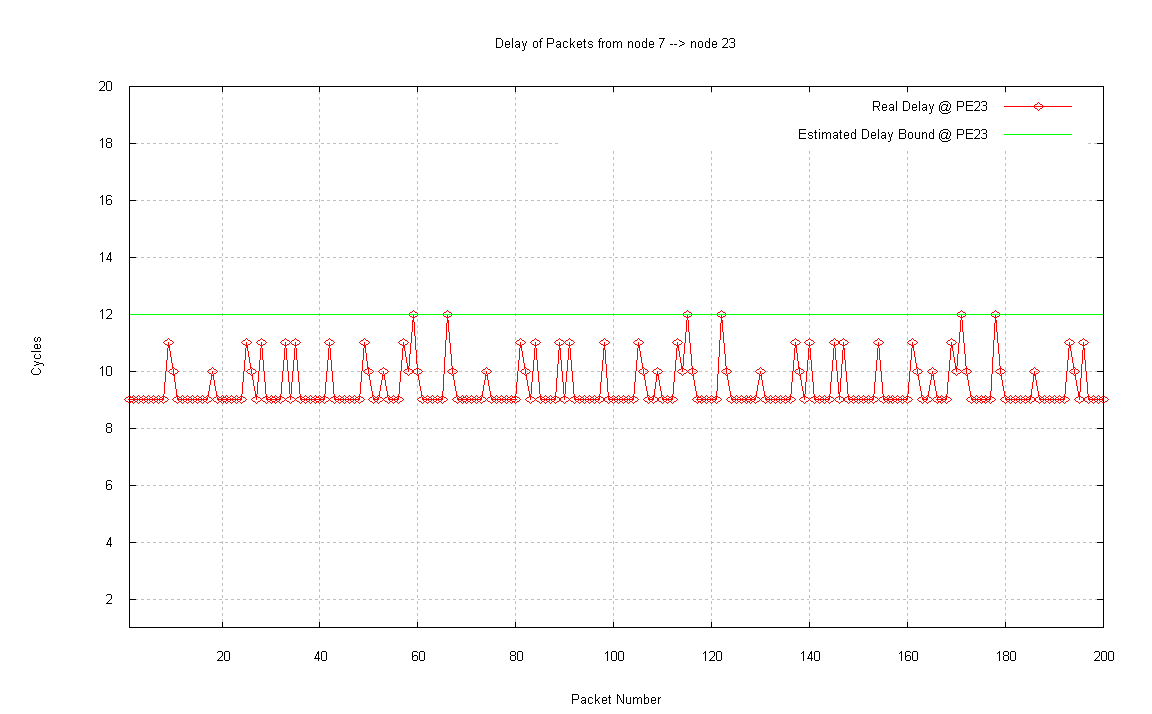
\includegraphics[width=8cm]{pics/PE23.png}
\caption[Flow from node 7 to node 23.]
{Real delay and estimated delay of real-time flow from node
7 to node 23}\label{fig:PE7PE23}
\end{figure}

\begin{figure}[htp]
\centering
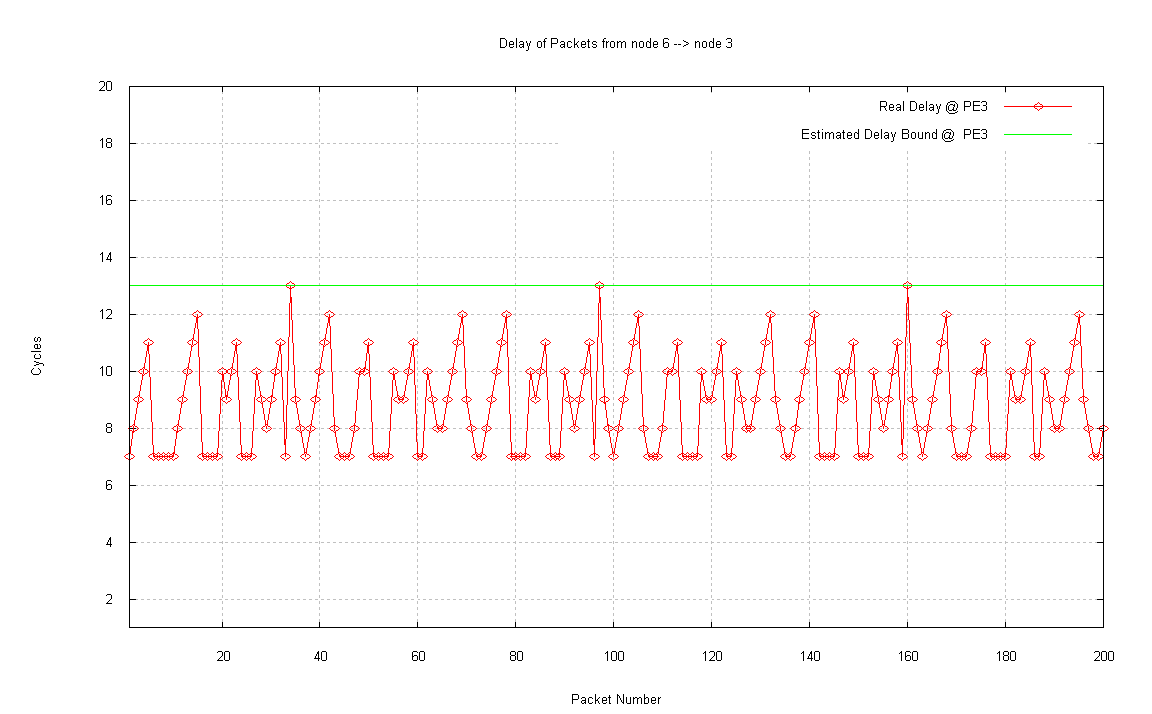
\includegraphics[width=8cm]{pics/PE3.png}
\caption[Three flows example.]
{Real delay and estimated delay of real-time flow from node
6 to node 3}\label{fig:PE6PE3}
\end{figure}

\begin{figure}[htp]
\centering
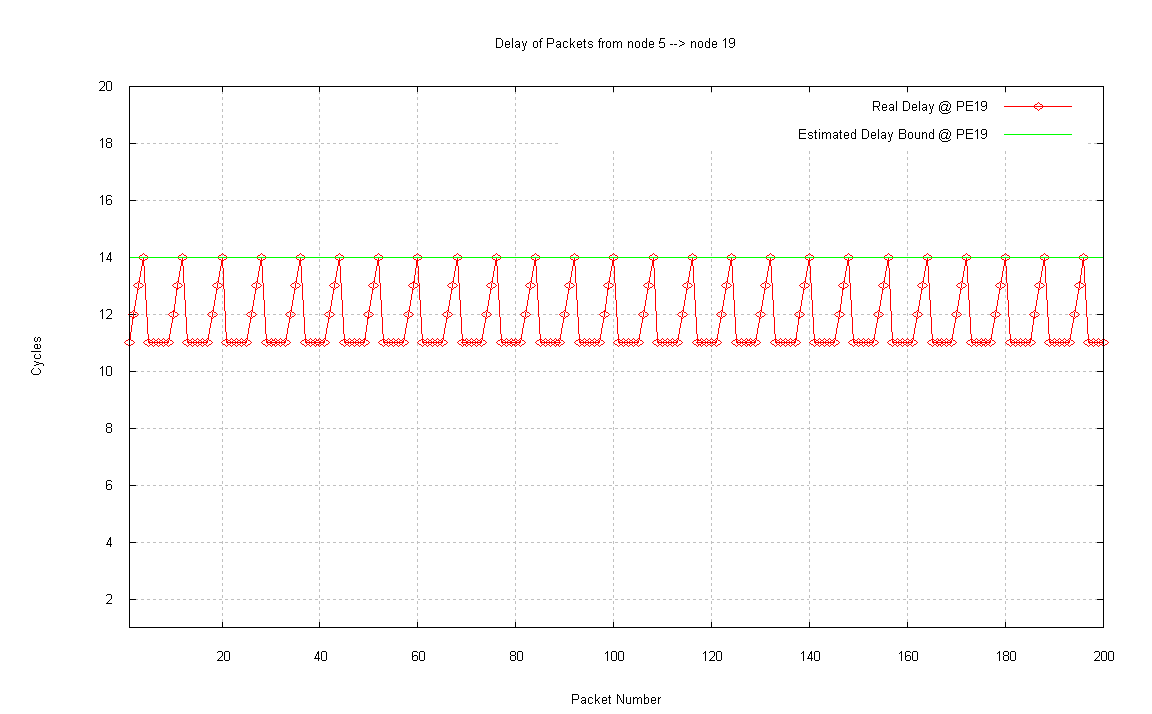
\includegraphics[width=8cm]{pics/PE19.png}
\caption[Three flows example.]
{Real delay and estimated delay of real-time flow from node
5 to node 19}\label{fig:PE5PE19}
\end{figure}

As we can see that the three flows interact with one another yet the delay of a
packet is never greater than the estimated delay bound. And the delay of these
flows is much lower than the average delay in a best-effort network like
this (Noxim original implementation), which is about more than {\em 5000}
cycles.

\section{Conclusion and Future Work}
We have shown a network on chip model for critical applications supposed to be
suitable for multi-core and many-core architecture. We suppose that message
passing programming model like MPI can benefit from this explicit message
delay scheme since we can reduce and predict the synchronization between
processing cores. Critical applications like air plane control can utilize the
development of multi-core since we can verify the delay communication between
processing elements.

In future, we will find different routing algorithms to optimize and balance a
network and we can incorporate multiple PRET processors ~\cite{LicklyPRET} into
a real-time multi-core system.

\bibliography{RTNoC}
\bibliographystyle{plain}

\end{document}
